\chapter{Implementation}
\label{cha:Implementation}

\section{Generalising the Codebase}
\label{sec:Generalising the Codebase}
The simulators created for this project were created partly using the AIM simulator codebase \citep{AIMWebsite}. We wanted to expand the simulator so that it could run AV simulations in situations other than 4-way intersections. To do this we needed to generalise the AIM codebase so that new developers could add simulators with very little effort, however, we also needed to ensure that these changes would not affect the functionality of the AIM simulator. \newtext{Compatibility between different simulations was one of the main project constraints. As such, I worked with Rebecca Milligan, who is also working on AV simulations in her car park management project, to ensure that we had a strong general codebase to develop from.}

To generalise the codebase we refactored key classes into separate general and AIM specific classes. The general classes can be expanded to create other simulator specific classes, whilst the AIM specific classes maintain the functionality of the original simulator. This helps to reduce code duplication when developing new simulators.

All class diagrams were created using IntelliJ IDEA 15.0.3 internal diagram tool. Figure \ref{fig:classDiagramKey} provides a key for understanding these diagrams.

\begin{figure}[htb]
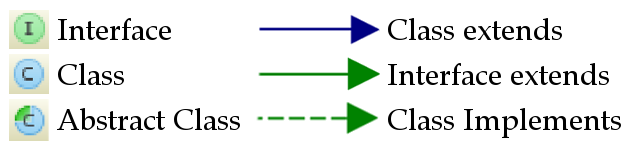
\includegraphics[width=\textwidth]{classDiagrams/classDiagramKey.png}
\caption{Key for the class diagrams in this report.}
\label{fig:classDiagramKey}
\end{figure}

\newtext{Refactoring the AIM codebase was more difficult that originally expected and many changes were made. For brevity, I have only described one of the key parts of the refactor, changing the class structure for classes in \emph{aim4.vehicle}. Appendix \ref{sec:Generalising the Codebase Appendix} provides detailed coverage of both this change, and changes made to some of the other areas of the AIM codebase.}

\todo{Describe this change}.

\section{Drivers}
\label{sec:Drivers}


\section{Testing}
\label{sec:Testing}

\subsection{Unit Testing}
\label{subsec:Unit Testing}
Unit tests were mostly used to ensure getter and setter methods worked as expected. However, some unit tests were used to verify the behaviour of classes. To do this I used Mockito \citep{MockitoWebsite} to mock the behaviour of objects used by the test class so that I could prompt the test class into producing the expected results.

\subsection{Integration Tests}
\label{subsec:Integration Tests}

